\chapter{Wstęp teoretyczny}\label{cha:pierwszyDokument}

%---------------------------------------------------------------------------

\section{Opis algorytmu ewolucji różnicowej}\label{sec:strukturaDokumentu}


Algorytm ewolucji różnicowej jest rodzajem heurystyki, a więc rodzajem algorytmu dla którego znalezione rozwiązanie nie jest objęte gwarancją bycia rozwiązaniem optymalnym. Metod heurystycznych używa się w sytuacji gdy przestrzeń potencjalnych rozwiązań jest zbyt duża iż nie jest możliwe w dostatecznie krótkim czasie przebadanie wszystkich  potencjalnych rozwiązań w celu znalezienia tego najlepszego. Algorytmy ewolucyjne są jednym z narzędzi służących do ukierunkowania procesu poszukiwań poprzez zastosowanie technik probabilistycznych, a co za tym idzie służących do usprawnienia rozwiązywania wspomnianej wyżej sytuacji. W większości przypadków, przy odpowiednim doborze parametrów rozwiązanie będące wynikiem działania algorytmu ewolucyjnego jest zarazem rozwiązaniem najbardziej optymalnym, nie mniej jednak zależność ta nie występuje  we wrzystkich przypadkach.

Swoim działaniem algorytmy ewolucyjne przypominają zjawisko ewolucji biologicznej a kolejne etapy algorytmu stanowią operacje będące odpowiednikami zjawisk typowych dla świata przyrody, a więc zjawiska selekcji, mutacji oraz krzyżowania. Inspiracja zasadą doboru naturalnego sprowadza się do  kierowania się ideą iż tylko najlepiej przystosowane osobniki mają szanse na przeżycie i to one powinny zapoczątkowywać istnienie nowych co raz to lepszych osobników potomnych, które to z koleji tworzą nowe mocniejsze populacje. Dzięki temu algorytm ewolucyjny tworzy stopniowo coraz lepsze rozwiązania i może służyć on do rozwiązywania problemów optymalizacyjnych.

Obecnie w skład algorytmów ewolucyjnych wchodzą między innymi algorytmy genetyczne, programowanie genetyczne czy też programowanie ewolucyjne. Jednak jeszcze w latach sześćdziesiątych istniały i rozwijały się one niezależnie od siebie jako oddzielne wersje wcielające w życie darwinowską zasadę doboru naturalnego. Dopiero od początku lat dwudziestych strategie ewolucyjne, algorytm genetyczny, programowanie ewolucyjne i programowanie genetyczne zaczęły być traktowane jako różne formy tej samej techniki określane wspólnym mianem algorytmów ewolucyjnych.

\subsection{Optymalizacja lokalna i globalna}

Problem optymalizacji może zostać w ogólności przedstawiony jako problem mający na celu znalezienie takiej wartości x w danym zbiorze X, dla której funkcja f(x) będąca funkcją celu, a więc funkcją mierzącą cel który ma zostać osiągnięty, przyjmuje najkorzystniejszą wartość. Wartość najkorzytstniejsza może być interpretowana w zależności od intencji jako minimum bądź też maksimum danej funkcji f(x). Minima i maksima są zbiorowo nazywane ekstremami odpowiednio globalnymi bądź lokalnymi.\\

Niech R oznacza zbiór wszystkich rozwiązań obranego problemu. Punkt x* w przestrzeni R jest minimum globalnym, jeśli dla każdego x należącego do R zachodzi zależność taka, że:
$$
 f(x*) \le f(x).
$$
Co można zapisać :
$$
x = x*   \Leftrightarrow   \forall x \in R,    f(x*)\le f(x)
$$
W takiej sytuacji x* jest optimum globalnym określającym najmniejszą wartość w całej dziedzinie. Nie mniej jednak łatwiejszym do znalezienia, rozwiązania i częściej formułowanym problemem jest zadanie określające minimum lokalne. Problem sprowadza się do znalezienia takiego $x_{1} $ dla którego 
$$
f(x_{1}) \le f(x_{1} + t), t >0
$$
gdzie $x_{1} + t $ są punktami otaczającymi $x_{1}$.
Można to zdefiniować w następujący sposób:
$$
x = x_{1} \Leftrightarrow f(x_{1}) \le f(x_{1} + t), t \ne 0
$$

Na rysunku \ref{minmax} zaznaczone są ekstrema funkcji spośród których możemy wyróżnić ekstrema lokalne oraz globalne. Odpowiednio punkty:\\

\begin{itemize}
\item A, C, E są maksimami lokalnymi,
\item G jest maksimum globalnym,
\item B, F są minimami lokalnymi,
\item D jest minimum globalnym
\end{itemize}

\begin{figure}[h!]
\begin{center}
		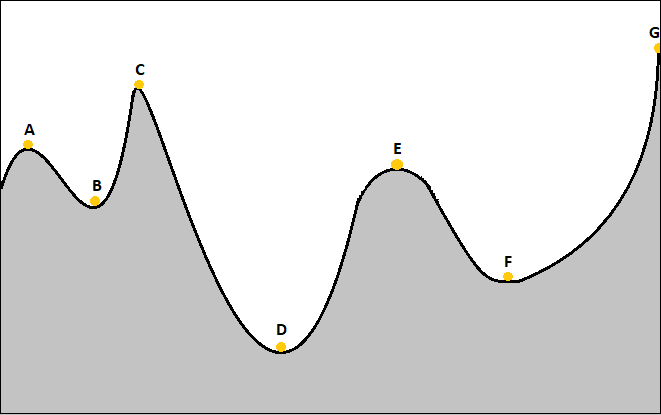
\includegraphics[scale=0.6]{../../../../Screeny/mixmax.png}
		\caption{Przebieg funkcji wraz z zaznaczonymi ekstremami}
		\label{minmax}		
\end{center}	
\end{figure}

Większość metod optymalizacyjnych ma zasięg lokalny, co znaczenie utrudnia poszukiwanie rozwiązania problemu jako, że algorytmy kończą swoje dzialanie w chwili gdy wartość funkcji celu osiągnie wartość ekstremum lokalnego. Powodem tych problemów jest zależność metod optymalizacyjnych od pochodnych funkcji, które to z koleji nie są wystarczająco odporne na nieciągłości czy też rozległe wielomodalności.
\par

\subsection{Podstawowe pojęcia}
W terminologi algorytmów genetycznych używa isę następująch pojęć zapożyczonych z genetyki naturalnej:\\

\textbf{Osobnik} - podstawowa jednostka charakteryzująca się pewnym przystosowaniem do środowiska w którym żyje czego miarą jest wartość funkcji celu obliczona dla tego osobnika. Dany osobnik jest wektorem liczb rzeczywistych będącym jednocześnie potencjalnym rozwiązaniem całego problemu optymalizacji.

\textbf{Populacja} - zbiór osobników ulegający zmianie w kolejnych iteracjach algorytmu jako, że słabsze osobniki są zastępowane przez nowe, lepiej przystosowane.

\textbf{Genotyp} - zbiór informacji przypisany do każdego osobnika indywidualnie, opisujący proponowane rozwiązanie problemu optymalizacyjnego.

\textbf{Fenotyp} - zbiór cech osobnika podlegających ocenie funkcji przystosowania.

\textbf{Chromosom} - jest to uporządkowany ciąg genów, który inaczej nazywany jest łańcuchem. W chromosomie zakodowany jest fenotyp i ewentualnie pewne informacje pomocnicze dla algorytmu genetycznego.

\textbf{Gen} - jest to pojedyńczy element chromosomu.

\textbf{Grupa rozrodcza} - zbiór osobników słóżących jako podstawa do utworzenia osobnika potomnego.

\textbf{Funkcja celu} - funkcja pozwalająca określić miarę przystosowania i jakość konkretnego osobnika z punktu widzenia rozwiązywanego problemu. Jako argument przyjmuje ona wektor będący odpowiednikiem osobnika.

\textbf{Funkcja dopasowania} - jest to funkcja stanowiąca modyfikacje funkcji celu tak aby zachować zależność iż im większa wartość funkcji dopasowania dla danego osobnika tym osobnik jest lepszy.

\textbf{Selekcja} - technika mająca na celu wybór osobników, które przedostaną się do grupy rozrodczej tworzącej potomstwo.

\textbf{Mutacja} - technika mająca na celu utworzenie nowego osobnika na podstawie osobników znajdujących się w grupie rozrodczej .

\textbf{Krzyżowanie} - technika mająca na celu utworzenie nowego osobnika na podstawie osobnika wynikowego mutacji oraz osobnika z aktualnej populacji.

\textbf{Operacje genetyczne} - zbiór operacji takich jak selekcja, mutacja, krzyżowanie.

\subsection{Pseudokod}
\par
 Większość algorytmów optymalizacyjnych stosuje procedure postępowania w której to z każdym krokiem działania algorytmu coraz bardziej zbliżamy się do rozwiązania optymalnego. Algorytmy tego typu zazwyczaj rozpoczynają poszukiwanie startując z konkretnego punktu, a następnie po uwzglednieniu dodatkowych informacji przemieszczają się dalej dochodząc po wielu iteracjach do rozwiązania końcowego.\\
\par
 W przypadku algorytmu ewolucyjnego początkiem jego działania jest utworzenie pierwszej populacji osobników będących pierwszymi potencjalnymi rozwiązaniami problemu. W każdej iteracji osobniki są poddawane ocenie zgodnie z przyjętą odgórnie funkcją celu. Następnie w zależności od przyjętej metody przeprowadzana jest selekcja w wyniku której otrzymujemy grupę rozrodczą. Grupa rozrodcza stanowi podstawę do przeprowadzenia operacji genetycznych jakimi są mutacja oraz krzyżowanie. Operacja mutacji dokonuje przekształceń genetycznych, na jednostce bądź grupie, w wyniku których powstaje nowy osobnik. Poddawany jest on operacji krzyżowania. Dopiero wynik tych dwóch operacji daje rezultat w postaci osobnika potomnego, którego współczynnik przystosowania zostaje oceniony. W sytuacji gdy będzie on większy od współczynnika przystosowania osobnika z obecnej populacji, nastąpi ich podmiana. Osobnik potomny zajmie w populacji miejsce poprzednika tworząc tym samym nową populacje a więc podstawę do rozpoczęcia nowej iteracji algorytmu. Warunkiem zakończenia algorytmu może być na przykład brak zmienności wyniku w kolejnych n iteracjach, bądź też osiągnięcie zadawalającego poziomu przystosowania.\\
\par
Opisane powżej zależności można zaprezentować w postaci schematu algorytmu przedstawionego na \ref{algo}.

\begin{figure}[h!]
\begin{center}
		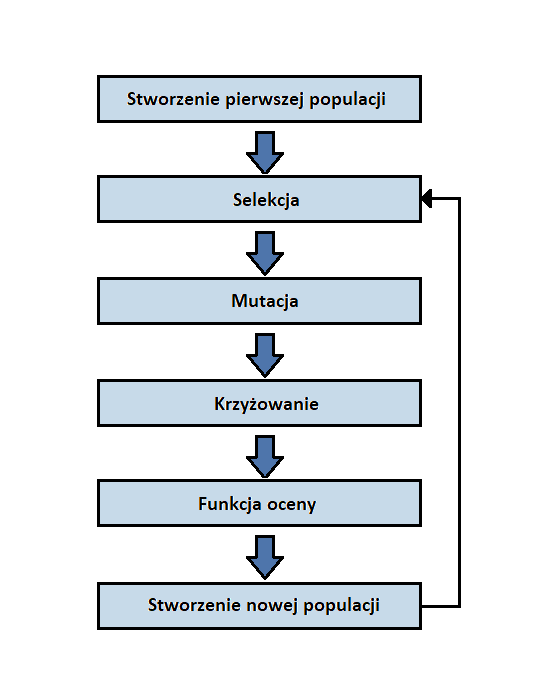
\includegraphics[scale=0.8]{../../../../Screeny/algo.png}
		\caption{Schemat algorytmu genetycznego}
		\label{algo}		
\end{center}	
\end{figure}

Dobór metod selekcji, mutacji czy też krzyżowania nie może zostać jednoznacznie określony i być uniwersalny dla wszystkich problemów które ma on rozwiązywać. Poprawność i jakość działania metod jest ściśle zależna od charakteru rozwiązywanego problemu. Z tego również względu w niektórych przypadkach konieczne jest dokonanie zmian w klasycznym algorytmie ewolucyjnym, w wyniku czego mamy doczynienia ze zmodyfikowanym algorytmem ewolucji różnicowej.
%---------------------------------------------------------------------------

\section{Opis kwadratowego zagadnienia przydziału}\label{sec:strukturaDokumentu}


